\documentclass{standalone}

\usepackage[dvipsnames]{xcolor}
\usepackage{tikz}
\usetikzlibrary{intersections}
\usepackage{fontspec}
\setmainfont[Scale=15.0]{Bilbo Swash Caps}%{HoltwoodOneSC}%{Roboto Slab-Black}

\Huge
\newlength{\inl}
\setlength{\inl}{1.1ex}%{0.66ex}

\begin{document}

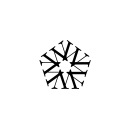
\begin{tikzpicture}[rotate=180]
	\node[rotate=180] at (90:\inl) {W};
	\node[rotate=252] at (162:\inl) {W};
	\node[rotate=324] at (234:\inl) {W};
	\node[rotate=36] at (306:\inl) {W};
	\node[rotate=108] at (18:\inl) {W};
	
%	\draw[line width=0.275ex] (120:2.25ex) -- (60:2.25ex) -- (0:2.25ex) -- (300:2.25ex) -- (240:2.25ex) -- (180:2.25ex) -- cycle;
%	\draw[line width=0.2ex] (0,0) circle (2.1ex);
\end{tikzpicture}

\end{document}